\documentclass[12pt]{article}
\usepackage[margin=1in]{geometry}
\usepackage{graphicx} % Required for inserting images
\usepackage{setspace}
\usepackage{float}
\usepackage{tabularx}
\usepackage{tabularray}
\usepackage[colorlinks]{hyperref}
\usepackage{placeins}
\usepackage{dcolumn}
\usepackage{booktabs}
\doublespace 

\begin{document}

\begin{center}
    \Large
    \textbf{Competition and Generic Drugs}
        
    \vspace{0.4cm}
    \large
    Evidence on Pharmaceutical Costs and Competition from Public Data Sources
        
       
    \vspace{0.9cm}
    \textbf{Abstract}
    
\end{center}

Pharmaceutical competition is central to debates about drug affordability and public spending. Building on research linking pharmaceutical competition and prices, I construct a panel from public Medicaid spending records for 2017--2021 to examine the association between reported drug manufacturer counts and spending per drug dosage unit. Across drug groups, one additional manufacturer is associated with 12.2\% lower spending per dosage unit and 8.7\% lower spending per claim, controlling for year fixed effects and prescription claim volume. Because manufacturers select which markets to enter, these estimates describe associations rather than causal effects of manufacturer entry.

\section{Introduction}
According to Rajkumar (2020), global spending on prescription drugs was expected to reach approximately \$1.3 trillion in 2020, with the United States accounting for \$350 billion. Rajkumar (2020) discusses the relationship between limited competition and high drug prices, while Kesselheim et al. (2016) emphasize the role of market exclusivity. Additionally, an FDA report by Conrad and Lutter (2019) reports median reductions in average manufacturer prices relative to pre-entry brand prices of 54\% with two generic manufacturers and 79\% with four.

For publicly financed programs such as Medicaid, drug spending has implications for both government budgets and access to treatment. In fiscal year 2021, Medicaid spent approximately \$80.6 billion on outpatient prescription drugs before manufacturer rebates and \$38.1 billion after rebates (MACPAC, 2024). This paper examines how reported manufacturer counts are associated with Medicaid spending per dosage unit.

Pharmaceutical policy faces a tension between encouraging innovation and maintaining affordable access to medicines. Developing new drugs involves substantial upfront costs and a risk of failure. One rationale for temporary market exclusivity is that the prospect of future profits encourages firms to undertake these investments. Generic competition, in turn, can lower the prices of existing medicines (Caves, Whinston, and Hurwitz, 1991).

\begingroup
\emergencystretch=1em
The literature also examines other determinants of pharmaceutical prices. Janssen Daalen et al. (2021) review studies of the determinants of drug prices. They find that retail drug prices vary substantially within and across countries and that the factors examined do not fully explain this variation. Determinants associated with lower retail prices include a higher market share of generics, central government purchasing, and price regulation. Determinants associated with higher retail prices include a higher market share of originator drugs and the presence of drug markups. They also identify particularly limited evidence on net drug prices, after discounts and rebates.
\par
\endgroup

An established literature examines generic entry and pharmaceutical pricing. Caves, Whinston, and Hurwitz (1991) examine prices and market shares following patent expiration and generic entry. Reiffen and Ward (2005) find lower generic prices in markets with more competitors and emphasize the role of expected market size in entry decisions. Grabowski and Vernon (1992) examine pricing strategies for branded and generic drugs following generic entry, including the role of brand loyalty.

Building on this literature, I construct a panel from public Medicaid spending records for 2017--2021 to examine the association between reported manufacturer counts and drug spending. I focus on spending per dosage unit, with spending per claim as a secondary outcome. Because manufacturers select which markets to enter, the estimates describe associations across drug groups rather than causal effects of manufacturer entry. Data from Mark Cuban's Cost Plus Drugs and NADAC provide supplementary descriptive evidence on pharmaceutical pricing. The Cost Plus analysis is presented in \hyperref[app:costplus]{Appendix~\ref*{app:costplus}}.

\section{Data Overview}
\subsection{Medicaid - Spending By Drug}
The first data source that I will discuss is Medicaid - Spending by Drug. This data contains Medicaid spending by drug from 2017 to 2021, along with other covariates. It represents national-level drug spending for Medicaid covered outpatient drugs, which are paid for by state Medicaid agencies. The spending measures include dispensing fees and are not reduced by manufacturer rebates (CMS, 2022). Over-the-counter drugs in the Medicaid State Drug Utilization data are not included, and drugs with fewer than 11 claims in the most recent year are also not included. The source contains 16,146 records, including records for individual manufacturers and records aggregating all manufacturers within a drug group. Each record contains annual information for 2017--2021. Reshaping these annual fields produces 80,730 rows, one for each record and year, including rows with missing annual values. After applying the sample restrictions described below, the analysis includes 12,740 observations across 3,244 drug groups.

In addition to the 16,146 total observations, each observation has a total of 36 covariates.
Four of the covariates are the brand name of the drug, the generic equivalent of that drug, the number of manufacturers for the drug, and the name of the manufacturer of the drug: these covariates are time-invariant during this period. In the analysis, I define drug groups by brand name and generic name. 30 of the covariates can be divided into 6 distinct spending/financial/counting features for each year in 2017-2021, inclusive. After transforming the data, the panel contains 11 covariates, including the year. For the analyses in this paper, the data is filtered to consider only the entries where the statistics are calculated by aggregating all of the manufacturers for a particular drug, the outlier flag is 0, and all the other statistics are greater than 0. The 11 covariates are described in \autoref{table:table6}; summary statistics are given in \autoref{summary:medicaid-all}, and \autoref{summary:medicaid-filtered} for the filtered data.

Outlier\_Flag is an indicator variable which represents if the drug is an outlier or not. A drug is labeled an outlier by the standard definition using the IQR, in addition to if it meets two other conditions. First, if there are fewer than 30 records associated with the drug from the initial data source, then it is flagged as an outlier. Second, average spending per dosage unit is calculated with and without outlier records. If these calculated amounts differ by 10 percent and \$1, then it is flagged as an outlier. The data used in this paper only includes observations for which Outlier\_Flag is 0 i.e. the observations are not outliers.

The last two features are percent change in average total spending per dosage unit from 2020-2021, and the annual growth rate in average total spending per dosage unit throughout 2017-2021, calculated using the compound annual growth rate. These are not used in the analyses. 

\subsection{Cost Plus Drugs}
The second data source that I will discuss is the data from Mark Cuban’s Cost Plus Drugs. To obtain the data, I web scraped the website page (legally) containing a list of all medications, using Selenium and BeautifulSoup packages in Python. The features are summarized by the following tables: 

This data has 442 observations, with two duplicate rows for two medications that each have two different dosage forms. This data has seven features: the medication name, brand name, dosage form, retail price, the Cost Plus price, the manufacturing cost, and the markup. Cost Plus sells only generic medication, so the medication name is the name for the generic. The retail price is the brand name price as reported by Cost Plus Drugs. According the website, this is calculated as "an average of retail prices across other pharmacies that is sourced from third-party data. This information is published at the time we add the medication so may not reflect current market prices." Therefore, some of the interpretation of this retail price must be taken with a grain of salt, but I choose to give the benefit of the doubt in this paper. 

The Cost Plus price is the price that Cost Plus is selling the medication for: it is calculated by factoring in manufacturing/labor/shipping costs in addition to a 15 percent markup. In particular, the Cost Plus price can be decomposed as 

$$ CP\_price = 1.15(manuf\_cost) + 3$$

where 3 is the pharmacy labor cost. Tax and shipping costs are not included. Features are describe in \autoref{table:table9}.

\subsection{NADAC}
The third data source is the NADAC data, which stands for the National Average Drug Acquisition Cost. This data contains 1,298,197 observations with 12 features. For the sake of avoiding the difficulties of interpreting the data during and soon after the COVID-19 pandemic, I specifically choose to use the NADAC data from 2019. Two of the features uniquely identify the drug: these are the National Drug Code description, which includes the drug name, strength, and dosage form; and the NDC, which is an 11 digit code. The features are summarized in \autoref{table:table11}, and summary statistics in \autoref{summary:nadac}.

\section{Competition and Costs}
The literature discussed above highlights the role of competition in pharmaceutical pricing. In this section, I outline the relevant economic theory and examine the association between reported manufacturer counts and Medicaid spending per dosage unit and per claim.
\subsection{Theoretical Background}
First, I will give a brief background on the relevant microeconomic theory \footnote{Sourced from Prof. Cecile Gaubert's notes from ECON 101A, Fall 2021.}, specifically the case of a monopoly. Let $y = D(p)$ be the demand curve which is a function of price $p$. In the case of a monopoly, the firm can choose $p$, in which case the quantity $y$ is determined by the demand. Alternatively, the quantity $y$ can be set by the firm, and so the price is determined as $p(y) = D^{-1}(y)$. The monopoly firm solves the maximization problem\footnote{Note that the profit function must be concave at the fixed point.}

\begin{equation}
\begin{array}{rrclcl}
\displaystyle \max_{y} & p(y)y - c(y).\\
\end{array}
\end{equation}

The first order condition is $$ p'(y)y + p(y) = c'_y(y)$$ where the $p'(y)y + p(y)$ is the marginal revenue, and $c'_y(y)$ is the marginal cost. In other words, the maximizing $y$ is at the intersection of the marginal revenue and marginal cost. 

Interestingly, the marginal revenue curve is significantly different than the marginal revenue in perfect competition, as marginal revenue is now a function of the quantity produced. In the case of perfect competition (and cases with more than one firm in general), an individual firm cannot totally control the market price: the market price is determined in part by strategic interactions with other competing firms. As the number of firms goes to infinity, the market price cannot be manipulated at all by any single firm: every firm is a price taker, and so the marginal revenue is a constant i.e. the market price. However, a monopoly can now set the market price by manipulating the quantity produced, and so has the freedom to choose the price such that its own economic profit is positive and maximized above all else. This manifests as "unnaturally" high prices.

One thing to note is that the marginal revenue curve lies below the demand curve, since it is the demand curve plus a negative number. Also, marginal revenue is a function of the quantity: in perfect competition, the price is given and is treated as a constant. The monopoly chooses the quantity which is at the intersection of the marginal revenue and marginal cost curve, but since the marginal revenue curve lies below the demand curve, the monopoly charges a price which is higher than the price in perfect competition, where the price in perfect competition is given by the intersection of marginal cost (the supply curve in perfect competition) and demand. This comparison suggests that greater competition can place downward pressure on prices, providing a theoretical motivation for examining the relationship between manufacturer counts and Medicaid drug spending.

\begin{figure}[H]
    \centering
    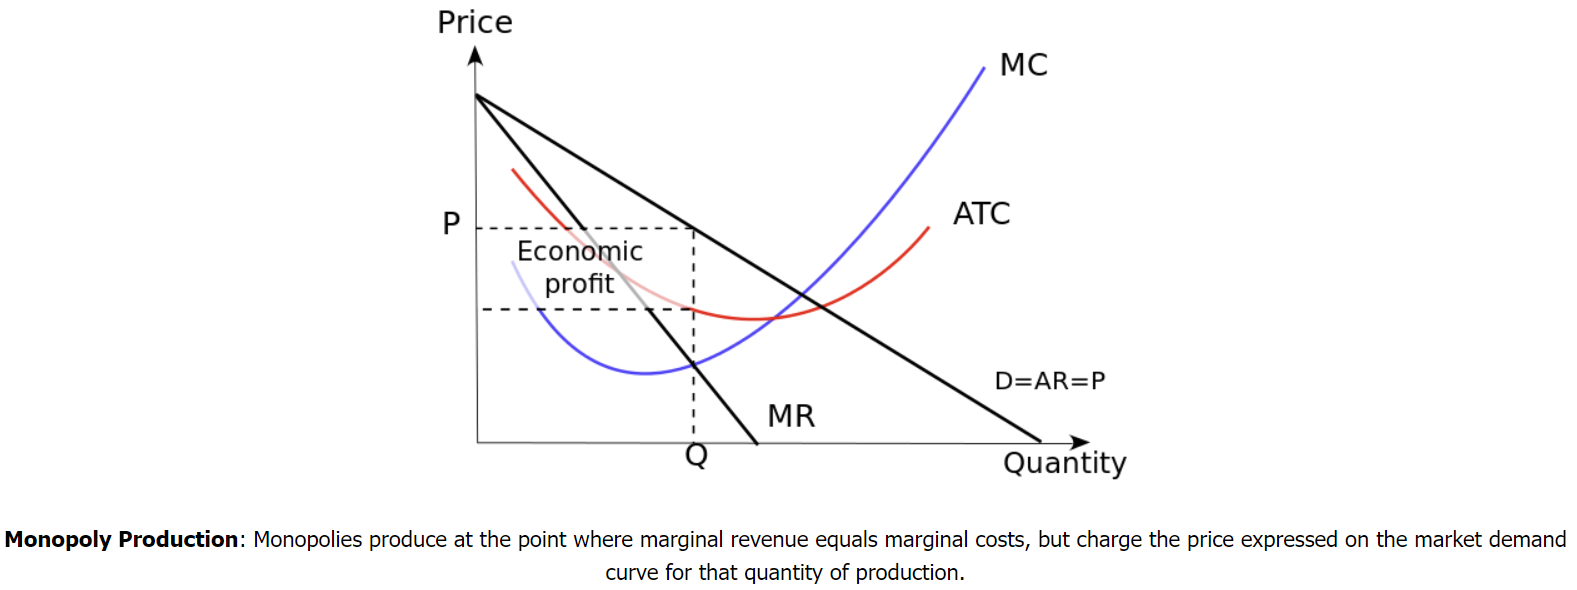
\includegraphics[width=16cm]{Screenshot (98).png}
    \caption{The monopoly chooses the price on the demand curve which correponds to the quantity at the intersection of MR = MC (LibreTexts).}
\end{figure}

\subsection{Empirical Analysis}
Using the filtered Medicaid data, I examine associations between the reported number of manufacturers and spending per dosage unit and per claim. For each outcome, I estimate regressions with year fixed effects, with and without log prescription claims.

We can first look at some preliminary results. If we group the data by the number of total manufacturers and average the spending per dosage unit, we can see an interesting relationship: 

\begin{figure}[H]
    \centering
    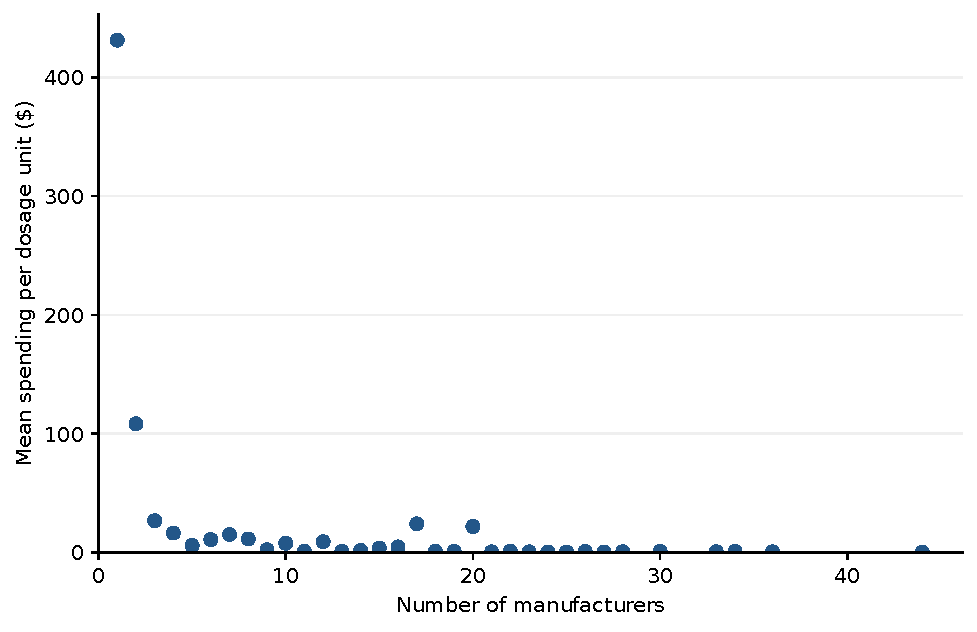
\includegraphics[width=13cm]{../analysis/output/figures/medicaid_mean_spending.pdf}
    \caption{Scatterplot of the mean average spending per dosage unit of drugs (y-axis), grouped by number of manufacturers (x-axis).}
\end{figure}

The plot shows that mean spending per dosage unit is substantially lower for drugs with two or three manufacturers than for drugs with one manufacturer. Mean spending remains comparatively low at higher manufacturer counts, although it does not fall consistently as the count increases. These descriptive comparisons across drug groups provide suggestive evidence of a negative association between manufacturer counts and drug spending, but may reflect factors other than manufacturer counts.

\newpage

\subsubsection{Regression Analysis}

For our regression specification, the outcomes are average spending per dosage unit and average spending per claim. For each outcome, I estimate

\[
Y_{it}=\alpha+\beta M_i+\gamma\log C_{it}+\lambda_t+u_{it},
\]
where $i$ denotes a drug group defined by brand name and generic name, $t$ denotes year, $Y_{it}$ is the natural logarithm of the spending outcome, $M_i$ is the reported manufacturer count, and $C_{it}$ is the number of prescription claims. Drugs with larger markets based on the number of prescription claims may attract more manufacturers and have different spending patterns. I include log prescription claims to adjust for differences in utilization across drug groups.

I estimate each model by unweighted pooled ordinary least squares, with and without the log-claims term. Year fixed effects $\lambda_t$ account for changes common to all drug groups, with 2017 as the reference year. Standard errors are clustered by drug group. The reported manufacturer count does not vary over time within a drug group in these data, so drug-group fixed effects would therefore absorb the manufacturer-count variable, preventing separate estimation of $\beta$. The manufacturer-count coefficient is estimated from differences across drug groups, conditional on the included controls.

% Generated by python -m analysis.run; do not edit.
\begin{table}[!htbp]
\centering
\caption{Manufacturer counts and log spending per dosage unit}
\label{table:table1}
\begin{singlespace}
\small
\begin{tabular*}{\linewidth}{@{\extracolsep{\fill}}lcc@{}}
\toprule
 & (1) & (2) \\
\midrule
Number of manufacturers & $-0.186^{***}$ & $-0.130^{***}$ \\
 & (0.008) & (0.011) \\
\addlinespace[2pt]
Log prescription claims &  & $-0.173^{***}$ \\
 &  & (0.022) \\
\addlinespace[2pt]
Constant & $2.221^{***}$ & $3.655^{***}$ \\
 & (0.062) & (0.185) \\
\addlinespace[2pt]
\midrule
Year fixed effects & Yes & Yes \\
Drug fixed effects & No & No \\
Observations & 12,740 & 12,740 \\
Drug groups & 3,244 & 3,244 \\
$R^2$ & 0.110 & 0.127 \\
Adjusted $R^2$ & 0.110 & 0.127 \\
\bottomrule
\end{tabular*}
\vspace{4pt}
\begin{minipage}{\linewidth}
\footnotesize
\textit{Notes:} OLS with year indicators for 2017--2021 (2017 omitted). Drug groups are brand-name/generic-name pairs. Standard errors in parentheses are clustered by drug group, with a finite-sample correction. Tests use a $t$ distribution with the number of groups minus one degrees of freedom. Manufacturer counts are time-invariant in these data.
$^{*}p<0.10$; $^{**}p<0.05$; $^{***}p<0.01$.
\end{minipage}
\end{singlespace}
\end{table}

\FloatBarrier

% Redundant total-spending table removed; associated prose awaits manual revision. 
\FloatBarrier

% Generated by python -m analysis.run; do not edit.
\begin{table}[!htbp]
\centering
\caption{Manufacturer counts and log spending per prescription claim}
\label{table:table3}
\begin{singlespace}
\small
\begin{tabular*}{\linewidth}{@{\extracolsep{\fill}}lcc@{}}
\toprule
\textit{Dependent variable:} & \multicolumn{2}{c}{\textbf{Log spending per claim}} \\
\addlinespace[3pt]
 & (1) & (2) \\
\midrule
Number of manufacturers & $-0.170^{***}$ & $-0.091^{***}$ \\
 & (0.007) & (0.008) \\
\addlinespace[2pt]
Log prescription claims &  & $-0.245^{***}$ \\
 &  & (0.016) \\
\addlinespace[2pt]
Constant & $5.795^{***}$ & $7.829^{***}$ \\
 & (0.049) & (0.143) \\
\addlinespace[2pt]
\midrule
Year fixed effects & Yes & Yes \\
Drug fixed effects & No & No \\
Observations & 12,740 & 12,740 \\
Drug groups & 3,244 & 3,244 \\
$R^2$ & 0.147 & 0.203 \\
Adjusted $R^2$ & 0.147 & 0.202 \\
\bottomrule
\end{tabular*}
\vspace{4pt}
\begin{minipage}{\linewidth}
\footnotesize
\textit{Notes:} OLS with year indicators for 2017--2021 (2017 omitted). Drug groups are brand-name/generic-name pairs. Standard errors in parentheses are clustered by drug group, with a finite-sample correction. Tests use a $t$ distribution with the number of groups minus one degrees of freedom. Manufacturer counts are time-invariant in these data.
All logarithms are natural.
$^{*}p<0.10$; $^{**}p<0.05$; $^{***}p<0.01$.
\end{minipage}
\end{singlespace}
\end{table}

\FloatBarrier

The regressions in column (1) of each table have a negative sign on the manufacturer-count coefficient, which is what we expect based on economic theory. In particular, an increase in one manufacturer is associated with a 16.9\% decrease in the average spend per dosage unit and a 15.6\% decrease in the average spend per claim, controlling for year effects.

As seen in the regression tables, adding the natural logarithm of total claims reduces the magnitude of the manufacturer-count coefficients and increases $R^2$ for both outcomes.

In regression (2) for average spend per dosage unit (\autoref{table:table1}), adding log(Tot\_Clms) increases $R^2$ from 0.110 to 0.127, and the adjusted $R^2$ is 0.127. Regression (2) indicates a negative association between the number of manufacturers and average spend per dosage unit. The coefficient on Tot\_Mftr is smaller in magnitude after adding log(Tot\_Clms), but remains statistically significant at the 1\% level using standard errors clustered by drug group. The coefficient indicates that one additional manufacturer is associated with a 12.2\% decrease in average spend per dosage unit, holding the included controls constant. Additionally, the coefficient on log(Tot\_Clms) is -0.173, indicating that a 1\% increase in total claims is associated with approximately a 0.173\% decrease in average spend per dosage unit, holding the other included variables constant. 

Looking at regression (2) for average cost per claim (\autoref{table:table3}), we can see that adding log(Tot\_Clms) increases $R^2$ from 0.147 to 0.203, and the adjusted $R^2$ is 0.202. One additional manufacturer is associated with an 8.7\% decrease in average spend per claim, holding the included controls constant. The manufacturer-count coefficient is statistically significant at the 1\% level. The coefficient on log(Tot\_Clms) is -0.245, indicating that a 1\% increase in total claims is associated with approximately a 0.245\% decrease in average spend per claim, holding the other included variables constant. This is a similar result to \autoref{table:table1}.

In summary, manufacturer counts are negatively associated with both measures of Medicaid drug spending, consistent with the economic theory and generic-entry literature discussed above. Manufacturers choose which drug markets to enter, and these decisions may depend on characteristics that also affect spending. The estimates therefore describe conditional associations across drug groups rather than causal effects of additional manufacturers. 

\section{Brand to Generic}
This final section will investigate differences between the NADAC of brand name drugs and their generic counterparts through a qualitative approach. I first separate the NADAC data into drugs with no generic counterpart, and the drugs where the rate is classified as generic in the NADAC. I then plot a density histogram of the natural logarithm of the NADAC Per Unit for both groups:

\begin{figure}[H]
    \centering
    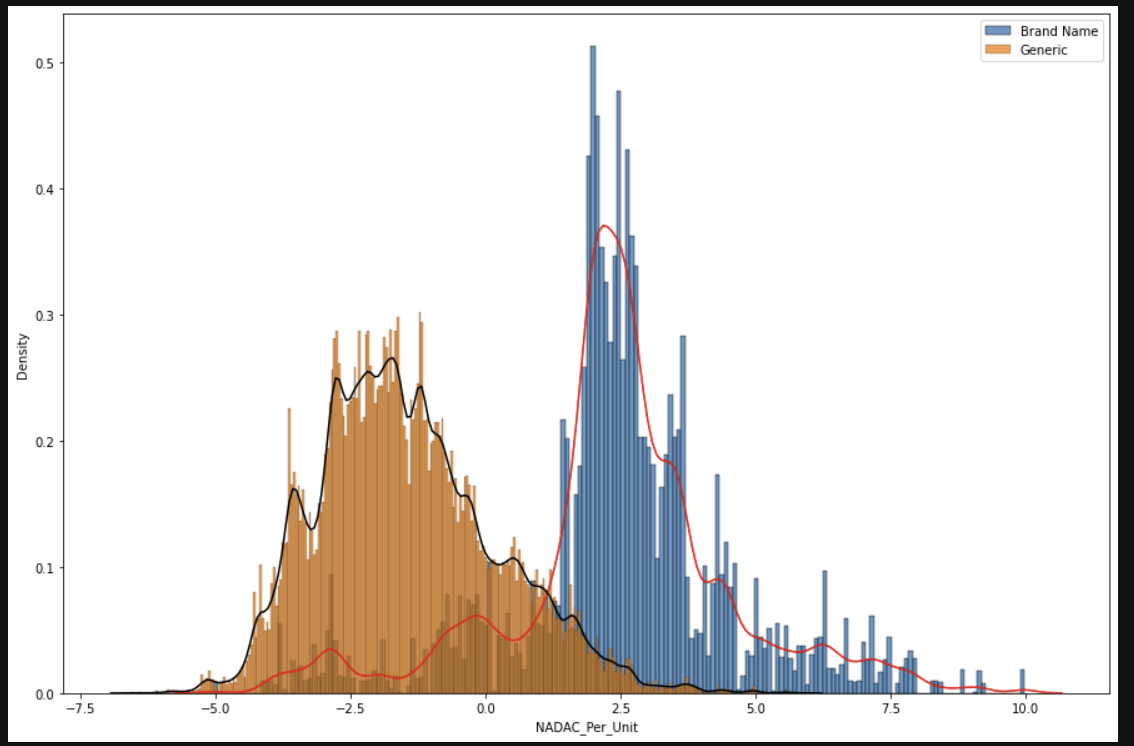
\includegraphics[width=13cm]{Screenshot (90).png}
    \caption{Histograms of log(NADAC Per Unit) of strictly brand name and generic drugs.}
    \label{fig:nadac-distributions}
\end{figure}
\FloatBarrier

Note that the brand name drugs distribution lies farther to the right along the x-axis, which indicates that brand name drugs are priced significantly higher on average compared to generics. The brand name density is also concentrated higher at a significantly higher NADAC per unit for brand name drugs: this tells us that brand name drugs are very consistently priced at a specific high “price range”. Additionally, we can also see that where most of the generic NADAC per unit values are, the brand name drugs are sparse in that same area. The lines drawn over the histograms are kernel density estimations (KDEs) of the respective distributions. Also note the fat tails of the brand name distribution, which indicates significantly high variance compared to the relatively symmetric and approximately normal distribution of the generic NADAC.

Now we consider brand name drugs which have had a corresponding generic introduced at some point. In total, there are 1286 of these drugs after accounting for duplicates. 

\begin{table}[!htbp] \centering 
  \caption{Summary Statistics - Brand Name with Generic} 
  \label{summary:nadac-paired} 
\begin{singlespace}
\small
\begin{tabular}{@{\extracolsep{5pt}}lccccc} 
\\[-1.8ex]\hline 
\hline \\[-1.8ex] 
Statistic & \multicolumn{1}{c}{N} & \multicolumn{1}{c}{Mean} & \multicolumn{1}{c}{St. Dev.} & \multicolumn{1}{c}{Min} & \multicolumn{1}{c}{Max} \\ 
\hline \\[-1.8ex]  
NADAC per unit & 1,286 & 16.173 & 41.481 & 0.005 & 471.559 \\ 
Corresponding generic NADAC per unit & 1,286 & 4.514 & 19.310 & 0.003 & 330.858 \\ 
nadac\_diff & 1,286 & $-$11.659 & 28.786 & $-$324.811 & 2.277 \\ 
nadac\_percent\_change & 1,286 & $-$0.696 & 0.292 & $-$0.999 & 1.679 \\ 
\hline \\[-1.8ex] 
\end{tabular}
\end{singlespace} 
\end{table} 
\FloatBarrier

The nadac\_diff is calculated by taking the difference between the corresponding generic NADAC per unit and the regular NADAC per unit. nadac\_percent\_change is calculated by taking nadac\_diff and dividing it by the corresponding NADAC per unit. One thing we can immediately notice is that, for most drugs in this comparison, the generic has a lower NADAC per unit than its brand-name counterpart. However, we can also see that there are some drugs for which the generic has a higher NADAC per unit than the brand-name counterpart.

\begin{table}[!htbp] \centering 
  \caption{Summary Statistics - Generic is More Expensive} 
  \label{summary:nadac-positive} 
\begin{singlespace}
\small
\begin{tabular}{@{\extracolsep{5pt}}lccccc} 
\\[-1.8ex]\hline 
\hline \\[-1.8ex] 
Statistic & \multicolumn{1}{c}{N} & \multicolumn{1}{c}{Mean} & \multicolumn{1}{c}{St. Dev.} & \multicolumn{1}{c}{Min} & \multicolumn{1}{c}{Max} \\ 
\hline \\[-1.8ex]  
NADAC per unit & 16 & 2.018 & 2.150 & 0.081 & 7.245 \\ 
Corresponding generic NADAC per unit & 16 & 2.493 & 2.257 & 0.116 & 7.686 \\ 
nadac\_diff & 16 & 0.474 & 0.656 & $-$0.027 & 2.277 \\ 
nadac\_percent\_change & 16 & 0.457 & 0.452 & 0.057 & 1.679 \\ 
\hline \\[-1.8ex] 
\end{tabular}
\end{singlespace} 
\end{table}
\FloatBarrier

For the drugs where the generic ends up more expensive, it is on average 45\% more expensive. However, since there are only 16 drugs, an increase in price in the generic is the exception rather than the rule. 

We can look at the distribution of the percent change:

\begin{figure}[H]
    \centering
    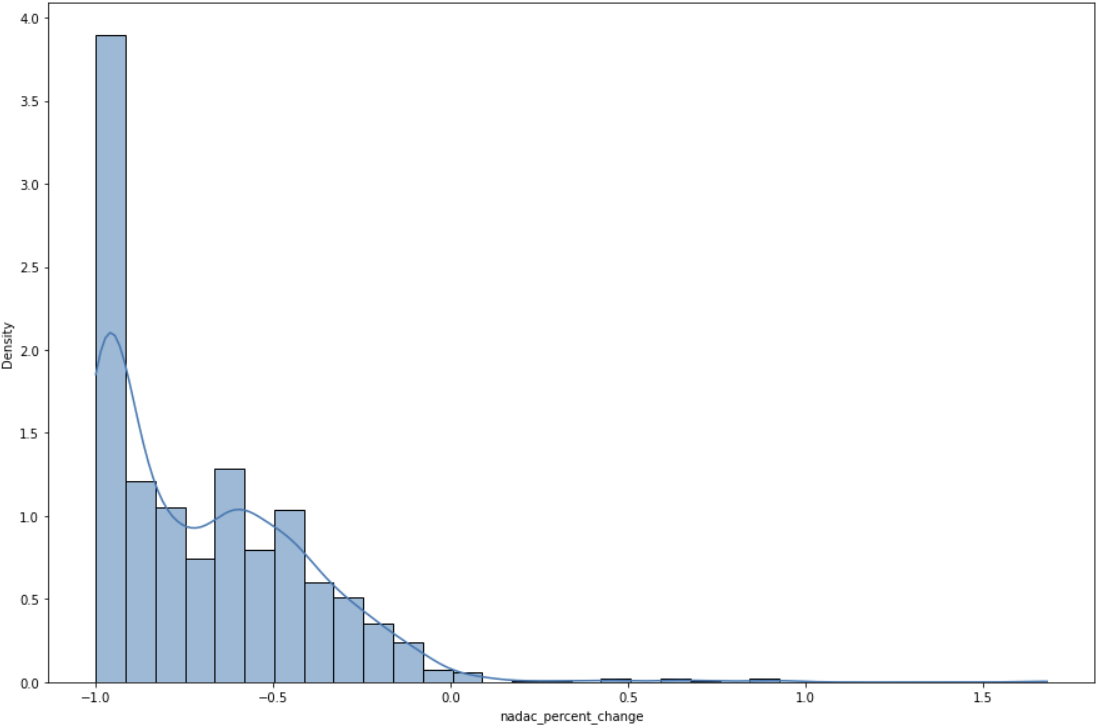
\includegraphics[width=13cm]{Screenshot (88).png}
    \caption{Density histogram of the percent change in NADAC}
    \label{fig:nadac-gap}
\end{figure}

We can see that, for a substantial proportion of drugs in this comparison, the generic NADAC per unit is approximately 90\% lower than the brand-name NADAC per unit.

In summary, the NADAC per unit of generic drugs tend to be significantly lower than those which are strictly brand name drugs. Additionally, the NADAC per unit for strictly brand name drugs has very high variance, while the NADAC per unit for generic drugs has relatively smaller variance. In a substantial proportion of the paired comparisons, generic NADAC per unit is at least 80\% lower than brand-name NADAC per unit, although some generics have higher acquisition costs. These comparisons describe acquisition-cost gaps in the 2019 data rather than changes following generic entry.

\section{Conclusion}
The Medicaid regressions show a negative association between manufacturer counts and average spending per dosage unit and per claim. Controlling for year fixed effects and log prescription claims, one additional manufacturer is associated with 12.2\% lower spending per dosage unit and 8.7\% lower spending per claim. These findings are consistent with the economic theory and generic-entry literature discussed above, but do not establish the causal effect of manufacturer entry.

The 2019 NADAC comparisons show that generic drugs generally have lower acquisition costs than brand-name drugs. This pattern is also present among drugs with a recorded generic counterpart. These gaps point to potential savings in acquiring medicines where suitable generic alternatives are available, although the comparisons do not measure savings for patients or Medicaid. The supplementary Cost Plus analysis in \hyperref[app:costplus]{Appendix~\ref*{app:costplus}} offers a complementary perspective on pharmaceutical pricing. Estimated manufacturing costs are associated with reported retail prices, but provide only a partial account of the price differences across drugs, as things such as demand and characteristics of competing products can also contribute to variation in retail prices.

The Medicaid findings point to competition as a potential means of improving drug affordability. If the observed relationship reflects competitive pressure, reducing obstacles to manufacturer entry could help contain spending on existing medicines. This possibility connects the results to the broader challenge of preserving incentives for pharmaceutical innovation while maintaining affordable access to treatment. For a publicly financed program, understanding this relationship is important for the cost of providing drug coverage. By constructing a panel from public Medicaid records, this paper contributes evidence on the relationship between market structure and Medicaid spending for drugs. Further research into why some drug markets attract more manufacturers than others could help establish when policies that encourage entry of manufacturers lead to lower spending. Understanding this could also help clarify how market characteristics shape entry decisions and inform research designs aimed at identifying the causal effect of entry on spending. Causal estimates would provide a stronger basis for evaluating policies that encourage competition.

\clearpage
% Include this file after the conclusion and before \appendix.
% Existing author--year citations in main.tex remain unchanged.
\begingroup
\hypersetup{urlcolor=black}
\section*{References}
\label{sec:references}

\begin{singlespace}
\begin{list}{}{
    \setlength{\leftmargin}{1.5em}
    \setlength{\itemindent}{-1.5em}
    \setlength{\itemsep}{0.75\baselineskip}
    \setlength{\parsep}{0pt}
}

\item
Boundless. n.d.
``Monopoly Production and Pricing Decisions and Profit Outcome.''
\textit{Economics}, Section 11.3. Social Sci LibreTexts.
\href{https://socialsci.libretexts.org/Bookshelves/Economics/Introductory_Comprehensive_Economics/Economics_(Boundless)/11:_Monopoly/11.03:_Monopoly_Production_and_Pricing_Decisions_and_Profit_Outcome}{Online textbook section}.

\item
Caves, Richard E., Michael D. Whinston, and Mark A. Hurwitz. 1991.
\href{https://www.brookings.edu/wp-content/uploads/1991/01/1991_bpeamicro_caves.pdf}{``Patent Expiration, Entry, and Competition in the U.S. Pharmaceutical Industry.''}
\textit{Brookings Papers on Economic Activity: Microeconomics} 1991: 1--66.

\item
Centers for Medicare \& Medicaid Services (CMS). 2022.
\href{https://data.cms.gov/sites/default/files/2022-01/DSD_MCD_R21_20220118_Methodology_WDDSE.pdf}{\textit{Medicaid Spending by Drug: Methodology}}.
January.

\item
Conrad, Ryan, and Randall Lutter. 2019.
\href{https://www.fda.gov/media/133509/download}{\textit{Generic Competition and Drug Prices: New Evidence Linking Greater Generic Competition and Lower Generic Drug Prices}}.
U.S. Food and Drug Administration, December.

\item
Gaubert, Cecile. 2021.
Lecture notes for ECON 101A, \textit{Microeconomics (Math Intensive)}.
University of California, Berkeley, Fall.

\item
Grabowski, Henry G., and John M. Vernon. 1992.
\href{https://doi.org/10.1086/467257}{``Brand Loyalty, Entry, and Price Competition in Pharmaceuticals after the 1984 Drug Act.''}
\textit{Journal of Law and Economics} 35(2): 331--350.

\item
Janssen Daalen, Jules M., Anouk den Ambtman, Mark van Houdenhoven,
and Bart J. F. van den Bemt. 2021.
\href{https://doi.org/10.1136/bmjopen-2020-046917}{``Determinants of Drug Prices: A Systematic Review of Comparison Studies.''}
\textit{BMJ Open} 11(7): e046917.

\item
Kesselheim, Aaron S., Jerry Avorn, and Ameet Sarpatwari. 2016.
\href{https://doi.org/10.1001/jama.2016.11237}{``The High Cost of Prescription Drugs in the United States: Origins and Prospects for Reform.''}
\textit{JAMA} 316(8): 858--871.

\item
Medicaid and CHIP Payment and Access Commission (MACPAC). 2024.
\href{https://www.macpac.gov/wp-content/uploads/2024/02/Policy-in-Brief-High-Cost-Drugs-FINAL-2.pdf}{\textit{High-Cost Drugs and the Medicaid Program: Evidence and Recommendations}}.
February.

\item
Mulcahy, Andrew W., and Vishnupriya Kareddy. 2022.
\href{https://www.rand.org/pubs/periodicals/health-quarterly/issues/v9/n3/07.html}{``Prescription Drug Supply Chains: An Overview of Stakeholders and Relationships.''}
\textit{RAND Health Quarterly} 9(3): 7.

\item
Rajkumar, S. Vincent. 2020.
\href{https://doi.org/10.1038/s41408-020-0338-x}{``The High Cost of Prescription Drugs: Causes and Solutions.''}
\textit{Blood Cancer Journal} 10: 71.

\item
Reiffen, David, and Michael R. Ward. 2005.
\href{https://doi.org/10.1162/0034653053327694}{``Generic Drug Industry Dynamics.''}
\textit{Review of Economics and Statistics} 87(1): 37--49.

\end{list}
\end{singlespace}
\endgroup


\clearpage
\appendix
\section{Manufacturing Costs: Mark Cuban's Cost Plus Drugs}
\label{app:costplus}
I will first investigate the relationship between manufacturing costs and pricing by looking at the Cost Plus data. 

I begin by attempting to isolate an estimate of the manufacturing cost from the CP\_price. As alluded to earlier, this is given by

$$ManufacturingCosts = \frac{CP\_price - 3}{1.15}$$.

Mulcahy and Kareddy (2022) also provide a brief outline of a general supply chain model for brand-name drugs at retail pharmacies:

\begin{figure}[H]
    \centering
    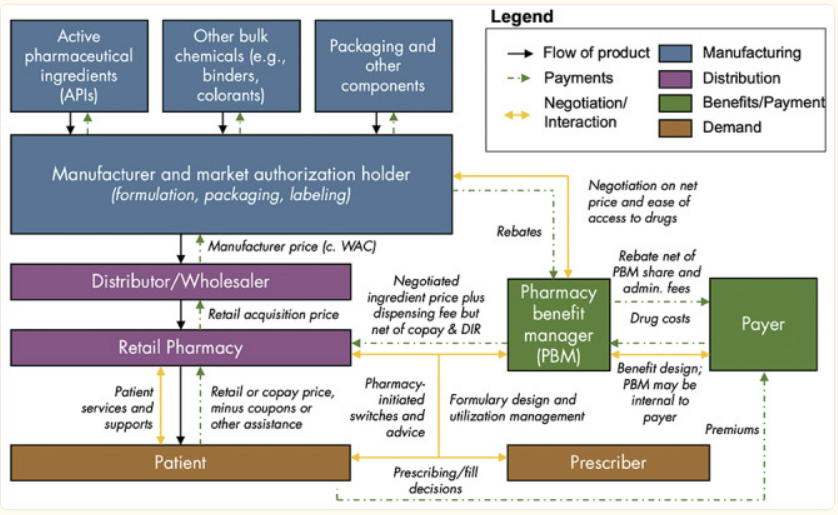
\includegraphics[width=14cm]{Screenshot (95).png}
    \caption{Mulcahy \& Kareddy (2022)}
    \label{figure:figure1}
\end{figure}

I assume that this calculation of manufacturing costs accounts for the costs reflected in the manufacturing cells (colored blue) in \autoref{figure:figure1}.

One place to start with regards to looking at the relationship between manufacturing costs and pricing is to look at the extent of a linear relationship between the manufacturing costs and the retail price given in the data. We can first start by looking at a scatterplot of the data: 

\begin{figure}[H]
    \centering
    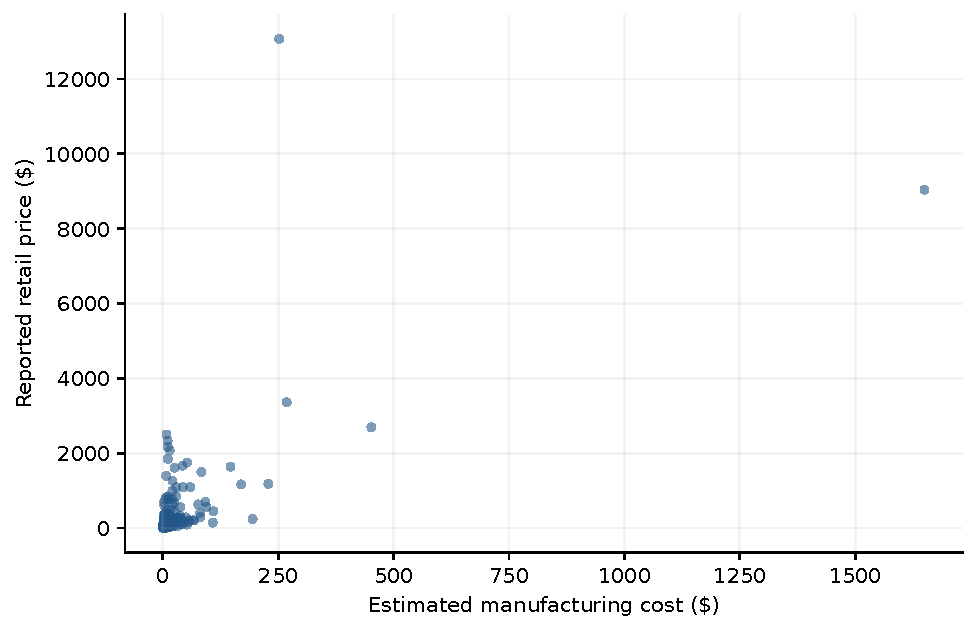
\includegraphics[width=13cm]{../analysis/output/figures/costplus_levels.pdf}
    \caption{Estimated manufacturing cost and reported retail price in the saved Cost Plus data.}
\end{figure}

The highly right skewed nature of both of the variables suggests that taking the natural logarithm of both of the variables may better reveal a linear relationship\footnote{Almost all of the variables in this paper have this relationship, so similar plots for other variables are omitted for brevity.}:

\begin{figure}[H]
    \centering
    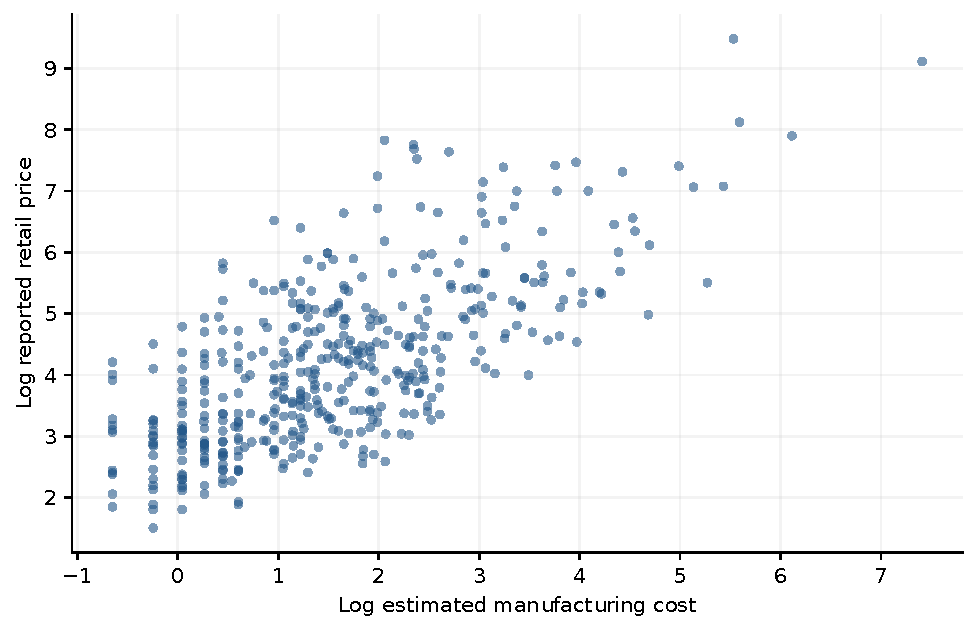
\includegraphics[width=13cm]{../analysis/output/figures/costplus_retail_log.pdf}
    \caption{Log reported retail price plotted against log estimated manufacturing cost.}
\end{figure}

Running an OLS regression on the variables above, we get

% Generated by python -m analysis.run; do not edit.
\begin{table}[!htbp]
\centering
\caption{\MakeUppercase{Estimated manufacturing cost and log reported retail price}}
\label{table:costplus-retail}
\begin{singlespace}
\small
\begin{minipage}{0.95\linewidth}
\begin{tabular*}{\linewidth}{@{\extracolsep{\fill}}lc@{}}
\toprule
 & \multicolumn{1}{c}{Log retail price} \\
\cmidrule(l){2-2}
 & (1) \\
\midrule
Log estimated manufacturing cost & $0.721^{***}$ \\
 & (0.034) \\
\addlinespace[5pt]
Constant & $3.068^{***}$ \\
 & (0.066) \\
\midrule
Observations & 442 \\
$R^2$ & 0.483 \\
Adjusted $R^2$ & 0.482 \\
\bottomrule
\end{tabular*}
\par\vspace{5pt}
\begin{minipage}{\linewidth}
\footnotesize
\raggedright
\textit{Notes:} OLS using the saved Cost Plus snapshot. HC3 heteroskedasticity-robust standard errors in parentheses; tests use the asymptotic normal distribution. Estimated manufacturing cost is $(\mathrm{CP\ price}-3)/1.15$.
All logarithms are natural.
$^{*}p<0.10$; $^{**}p<0.05$; $^{***}p<0.01$.
\end{minipage}
\end{minipage}
\end{singlespace}
\end{table}


The Cost Plus results suggest that manufacturing costs help explain retail-price differences, but provide an incomplete account of pricing. The coefficient of 0.721 indicates that a 1\% higher estimated manufacturing cost is associated with approximately 0.72\% higher reported retail price. The regression accounts for 48.3\% of the variation in log retail prices, leaving substantial differences unexplained by this cost measure. Manufacturing costs are inferred from the Cost Plus pricing rule and may not represent the production costs underlying the reported retail prices. Measurement error and differences across products could therefore contribute to the observed pattern. These results cannot distinguish the contribution of these alternative explanations or establish how prices respond when production costs change.

\section{Data Overview Tables}

\begin{table}[H]
\centering
\begin{singlespace}
\small
\begin{tabularx}{\linewidth}{@{}p{0.34\linewidth}X@{}}

\multicolumn{1}{c}{\textit{{Features}}} & \multicolumn{1}{c}{\textit{{Description}}} \tabularnewline 

\hline

Brnd\_\allowbreak{}Name & The brand name of the drug, if there is a brand name (trademarked name). Otherwise, the generic name is listed. \tabularnewline \hline

Gnrc\_\allowbreak{}Name & The name of the chemical compound which makes up the drug. \tabularnewline \hline

Tot\_\allowbreak{}Mftr & The total number of manufacturers for each drug. \tabularnewline \hline

Mftr\_\allowbreak{}Name & Name of the manufacturer of the drug. \tabularnewline \hline

Year & Year of the particular observation. \tabularnewline \hline

Tot\_\allowbreak{}Spndng & Total Medicaid spending for the corresponding drug and year. \tabularnewline \hline

Tot\_\allowbreak{}Dsg\_\allowbreak{}Unts & Total dosage units of the drug which are dispensed in the corresponding year. The dosage unit refers to the lowest dispensable amount for the corresponding drug. \tabularnewline \hline

Tot\_\allowbreak{}Clms & The total number of prescription fills for the drug, consisting of original prescriptions and refills. \tabularnewline \hline

Avg\_\allowbreak{}Spnd\_\allowbreak{}Per\_\allowbreak{}Dsg\_\allowbreak{}Unt\_\allowbreak{}Wghtd & This is the Medicaid spending divided by the total number of dosage units. This is weighted by the proportion of total claims with respect to different forms of the drug, such as different dosage strengths, forms, etc.\tabularnewline \hline

Avg\_\allowbreak{}Spnd\_\allowbreak{}Per\_\allowbreak{}Clm & Total Medicaid spending divided by the total number of prescription claims for the corresponding drug and year. \tabularnewline \hline

Outlier\_\allowbreak{}Flag & An indicator variable which equals 1 if the drug's statistics are affected by some form of outlier circumstances. Further details can be found below. \tabularnewline \hline

\end{tabularx}
\end{singlespace}
\caption{Description of the features in the Medicaid data.}
\label{table:table6}
\end{table}

% Generated by python -m analysis.run; do not edit.
\begin{table}[!htbp]
\centering
\caption{Summary statistics: Medicaid, unfiltered}
\label{summary:medicaid-all}
\begin{singlespace}
\small
\setlength{\tabcolsep}{4pt}
\begin{tabularx}{\linewidth}{@{}Xrrrrr@{}}
\toprule
Variable & $N$ & Mean & Std. dev. & Min. & Max. \\
\midrule
Manufacturers & 80,730 & 1.462 & 2.289 & 1.000 & 44.000 \\
Total spending (\$) & 67,807 & 10,840,301 & 59,961,216 & 0 & 2,730,141,376 \\
Dosage units & 67,807 & 8,401,479 & 309,329,351 & 0.045 & 56,150,332,658 \\
Prescription claims & 67,807 & 99,772 & 520,417 & 11.000 & 15,084,149 \\
Spending per dosage unit (\$) & 67,807 & 332.621 & 15,885 & 0 & 1,898,689 \\
Spending per prescription claim (\$) & 67,807 & 1,373 & 16,018 & 0 & 1,717,862 \\
\bottomrule
\end{tabularx}
\vspace{4pt}
\begin{minipage}{\linewidth}
\footnotesize
\textit{Notes:} All manufacturer-specific and Overall records, 2017--2021. Records for different manufacturers are not independent market totals.
Statistics use available observations; missing values are not replaced with zero. Large values are rounded to whole units; small positive values retain additional precision.
\end{minipage}
\end{singlespace}
\end{table}


% Generated by python -m analysis.run; do not edit.
\begin{table}[!htbp]
\centering
\caption{Summary statistics: Medicaid analysis sample}
\label{summary:medicaid-filtered}
\begin{singlespace}
\small
\setlength{\tabcolsep}{4pt}
\begin{tabularx}{\linewidth}{@{}Xrrrrr@{}}
\toprule
Variable & $N$ & Mean & Std. dev. & Min. & Max. \\
\midrule
Manufacturers & 12,740 & 3.338 & 4.789 & 1.000 & 44.000 \\
Total spending (\$) & 12,740 & 26,330,881 & 94,373,353 & 216.710 & 2,730,141,376 \\
Dosage units & 12,740 & 22,030,741 & 529,482,180 & 57.273 & 56,150,332,658 \\
Prescription claims & 12,740 & 251,271 & 1,039,414 & 36.000 & 15,084,149 \\
Spending per dosage unit (\$) & 12,740 & 283.404 & 1,699 & 0.0003285 & 39,360 \\
Spending per prescription claim (\$) & 12,740 & 2,098 & 7,256 & 0.895 & 187,154 \\
\bottomrule
\end{tabularx}
\vspace{4pt}
\begin{minipage}{\linewidth}
\footnotesize
\textit{Notes:} Overall records with no outlier flag and positive observed spending, dosage units, claims, both spending averages, and manufacturer count.
Statistics use available observations; missing values are not replaced with zero. Large values are rounded to whole units; small positive values retain additional precision.
\end{minipage}
\end{singlespace}
\end{table}


\begin{table}
\centering
\begin{singlespace}
\small
\begin{tabularx}{\linewidth}{@{}p{0.34\linewidth}X@{}}

\multicolumn{1}{c}{\textit{{Features}}} & \multicolumn{1}{c}{\textit{{Description}}} \tabularnewline 

\hline

medication & The generic name of the corresponding drug. Also notes the brand name counterpart. \tabularnewline \hline

brand\_\allowbreak{}name & The brand (trademarked) name of the corresponding drug. \tabularnewline \hline

form & The dosage form of the drug when purchased from the website. \tabularnewline \hline

retail\_\allowbreak{}price & The brand name price as reported by Cost Plus Drugs. According to the website, this is calculated as "an average of retail prices across other pharmacies that is sourced from third-party data. This information is published at the time we add the medication so may not reflect current market prices." \tabularnewline \hline

CP\_\allowbreak{}price & The sale price of the medication when purchasing from Cost Plus. \tabularnewline \hline

manuf\_\allowbreak{}cost & Estimate of the manufacturing costs of the drug. Method of calculation is discussed in the Manufacturing Costs and Pricing section. \tabularnewline \hline

markup & Percentage markup from the CP\_price to the retail\_price. Method of calculation is discussed in the Manufacturing Costs and Pricing section. \tabularnewline \hline

\end{tabularx}
\end{singlespace}
\caption{Description of the features in the Cost Plus Drugs data.}
\label{table:table9}
\end{table}

% Generated by python -m analysis.run; do not edit.
\begin{table}[!htbp]
\centering
\caption{Summary statistics: Cost Plus}
\label{summary:costplus}
\begin{singlespace}
\small
\setlength{\tabcolsep}{4pt}
\begin{tabularx}{\linewidth}{@{}Xrrrrr@{}}
\toprule
Variable & $N$ & Mean & Std. dev. & Min. & Max. \\
\midrule
Reported retail price (\$) & 442 & 229.526 & 838.190 & 4.500 & 13,067 \\
Cost Plus price (\$) & 442 & 22.543 & 98.288 & 3.600 & 1,900 \\
Estimated manufacturing cost (\$) & 442 & 16.994 & 85.468 & 0.522 & 1,650 \\
Constructed markup (\%) & 442 & 2,308 & 3,716 & 24.558 & 31,838 \\
\bottomrule
\end{tabularx}
\vspace{4pt}
\begin{minipage}{\linewidth}
\footnotesize
\textit{Notes:} Saved historical snapshot. Estimated manufacturing cost and markup are constructed from reported prices.
Statistics use available observations; missing values are not replaced with zero. Large values are rounded to whole units; small positive values retain additional precision.
\end{minipage}
\end{singlespace}
\end{table}


\begin{table}
\centering
\begin{singlespace}
\small
\begin{tabularx}{\linewidth}{@{}p{0.34\linewidth}X@{}}

\multicolumn{1}{c}{\textit{{Features}}} & \multicolumn{1}{c}{\textit{{Description}}} \tabularnewline 

\hline

NDC Description & Includes the name, strength, and dosage form of the particular drug. \tabularnewline \hline

NDC & 11 digit code which uniquely identifies the drug. Specifically, it is the NDC package code. \tabularnewline \hline

NADAC Per Unit & National Average Drug Acquistion Cost per unit. \tabularnewline \hline

Effective Date & The effective date of the NADAC entry for the drug. \tabularnewline \hline

Pricing Unit & The unit which the price is calculated with. “EA” stands for discrete units, such as pills. “ML” stands for milliliters, and “GM” stands for grams. \tabularnewline \hline

Pharmacy Type Indicator & The source of pharmacy survey data used for the NADAC. The only entry is "C/I", which stands for chain and independent pharmacies. This column does not give new information, since all entries are the same. \tabularnewline \hline

OTC & Indicates whether the drug is sold over-the-counter or not. "Y" means yes, "N" means no. \tabularnewline \hline

Explanation Code & Number from 1-10 which indicates how the NADAC was calculated. None are particularly problematic for this investigation, so I will omit the descriptions for brevity. \tabularnewline \hline

Classification for Rate Setting & Indicates whether the drug is considered brand (‘B’) or generic (‘G’) for the NADAC rate calculation process. Two other indicators specify further circumstances for brand name drugs: they are not problematic for this investigation. \tabularnewline \hline

Corresponding Generic Drug NADAC Per Unit & NADAC for the corresponding generic drug. The entry is NaN if there is no generic. \tabularnewline \hline

Corresponding Generic Drug Effective Date & The effective date of when the Corresponding Generic Drug NADAC Per Unit is assigned to a drug. This date may not correspond to the NADAC effective date for the generic drug. \tabularnewline \hline

\end{tabularx}
\end{singlespace}
\caption{Description of the features in the NADAC data.}
\label{table:table11}
\end{table}

\begin{table}[!htbp] \centering 
\addtolength{\tabcolsep}{-2pt}
  \caption{Summary Statistics (NADAC)} 
  \label{summary:nadac} 
\begin{singlespace}
\small
\begin{tabular}{@{\extracolsep{3pt}}lccccc}
\\[-1.8ex]\hline 
\hline \\[-1.8ex] 
Statistic & \multicolumn{1}{c}{N} & \multicolumn{1}{c}{Mean} & \multicolumn{1}{c}{St. Dev.} & \multicolumn{1}{c}{Min} & \multicolumn{1}{c}{Max} \\ 
\hline \\[-1.8ex] 
NADAC per unit & 1,298,197 & 10.529 & 240.682 & 0.001 & 21,513.920 \\ 
Corresponding generic NADAC per unit & 50,251 & 4.502 & 20.375 & 0.003 & 372.074 \\ 
\hline \\[-1.8ex] 
\end{tabular}
\end{singlespace} 
\end{table} 



\end{document}
